% Please use the skeleton file you have received in the
% invitation-to-submit email, where your data are already
% filled in. Otherwise please make sure you insert your
% data according to the instructions in PoSauthmanual.pdf
\documentclass{PoS}

\usepackage{tabularx}
\usepackage{xspace}

\newcommand{\fixme}[1]{\textbf{FIXME: #1}}    
\newcommand{\pd}{protoDUNE\xspace}

\title{The \pd-SP experiment and its prompt processing system}

\ShortTitle{The \pd-SP experiment and its prompt processing system}

\author{\speaker{Maxim Potekhin}\thanks{For the Deep Underground Neutrino Experiment Collaboration.}\\
        Brookhaven National Laboratory, USA\\
        E-mail: \email{potekhin@bnl.gov}}

%\author{Another Author\\
%        Affiliation\\
%        E-mail: \email{...}}

\abstract{
\noindent The Deep Underground Neutrino Experiment (DUNE) will employ a uniquely large % multi-kiloton
Liquid Argon Time Projection Chamber with four separate modules of 10kt fiducial mass each. Different modules will utilize
single and dual-phase Liquid Argon technologies. An experimental 
program (``protoDUNE'')  has been initiated which includes a beam and cosmic ray test of large-scale DUNE prototypes at CERN in 2018.
The volume of data to be collected by the protoDUNE single-phase detector will amount to a few petabytes
and the sustained rate of data sent to mass storage will be in the range of a few hundred megabytes per second.
The protoDUNE experiment requires substantial Data Quality Monitoring capabilities in order to ascertain the
condition of the detector and its various subsystems. To this end, a Prompt Processing system has been developed
which is complementary to Online Monitoring and is characterized by a lower bandwidth, scalable CPU resources
and end-to-end latency on the scale of a few minutes. We present the design of the protoDUNE Prompt Processing
system, the current status of its development and testing and issues related to its interfaces and deployment.

}

\FullConference{EPS-HEP 2017, European Physical Society conference on High Energy Physics\\
		5-12 July 2017\\
		Venice, Italy}

\begin{document}

\section{Overview of the protoDUNE-SP experiment}
The \pd program aims to validate various aspects of the DUNE  Liquid Argon Time Projection Chamber (LArTPC)  technology 
before proceeding with the construction of the large-scale principal DUNE detectors at the Sanford Underground Research
Facility \cite{cdrVol1, cdrVol4}. It  is designed to make a series of measurements of the interactions of
charged particles in the Liquid Argon medium.  These measurements will be performed with a dedicated test
beam line  at the CERN SPS accelerator complex which will allow the transport of beam particles from $\sim$0.5 GeV/c
up to 7 GeV/c. The run plan also includes a large number of cosmic ray triggers. The program includes
two separate large LArTPC prototypes, one based on a ``single-phase'' (liquid) technology and
the other based on a ``dual-phase'' (liquid/gaseous) TPC readout technology.
Both detectors are placed in an extension of the CERN North Area Experimental Hall and  scheduled
to take data in 2018. The general layout of the experimental area is shown in Fig.\,\ref{fig:np02np04}, with
the single-phase detector seen as a cubic structure on the right.

Located in the vicinity of the detectors will be enclosures which will house the elements of the local computing infrastructure
(including Data Acquisition, Online Buffer etc). These enclosures are shown schematically as yellow blocks in the
upper-right portion of Fig.\,\ref{fig:np02np04}, and they will have a dedicated 20 Gb/s
network connection over optical fiber to the CERN central storage facilities.

%%%%%%%%%%%%%%%%%%%%%%%%
\begin{figure}[tb]
\centering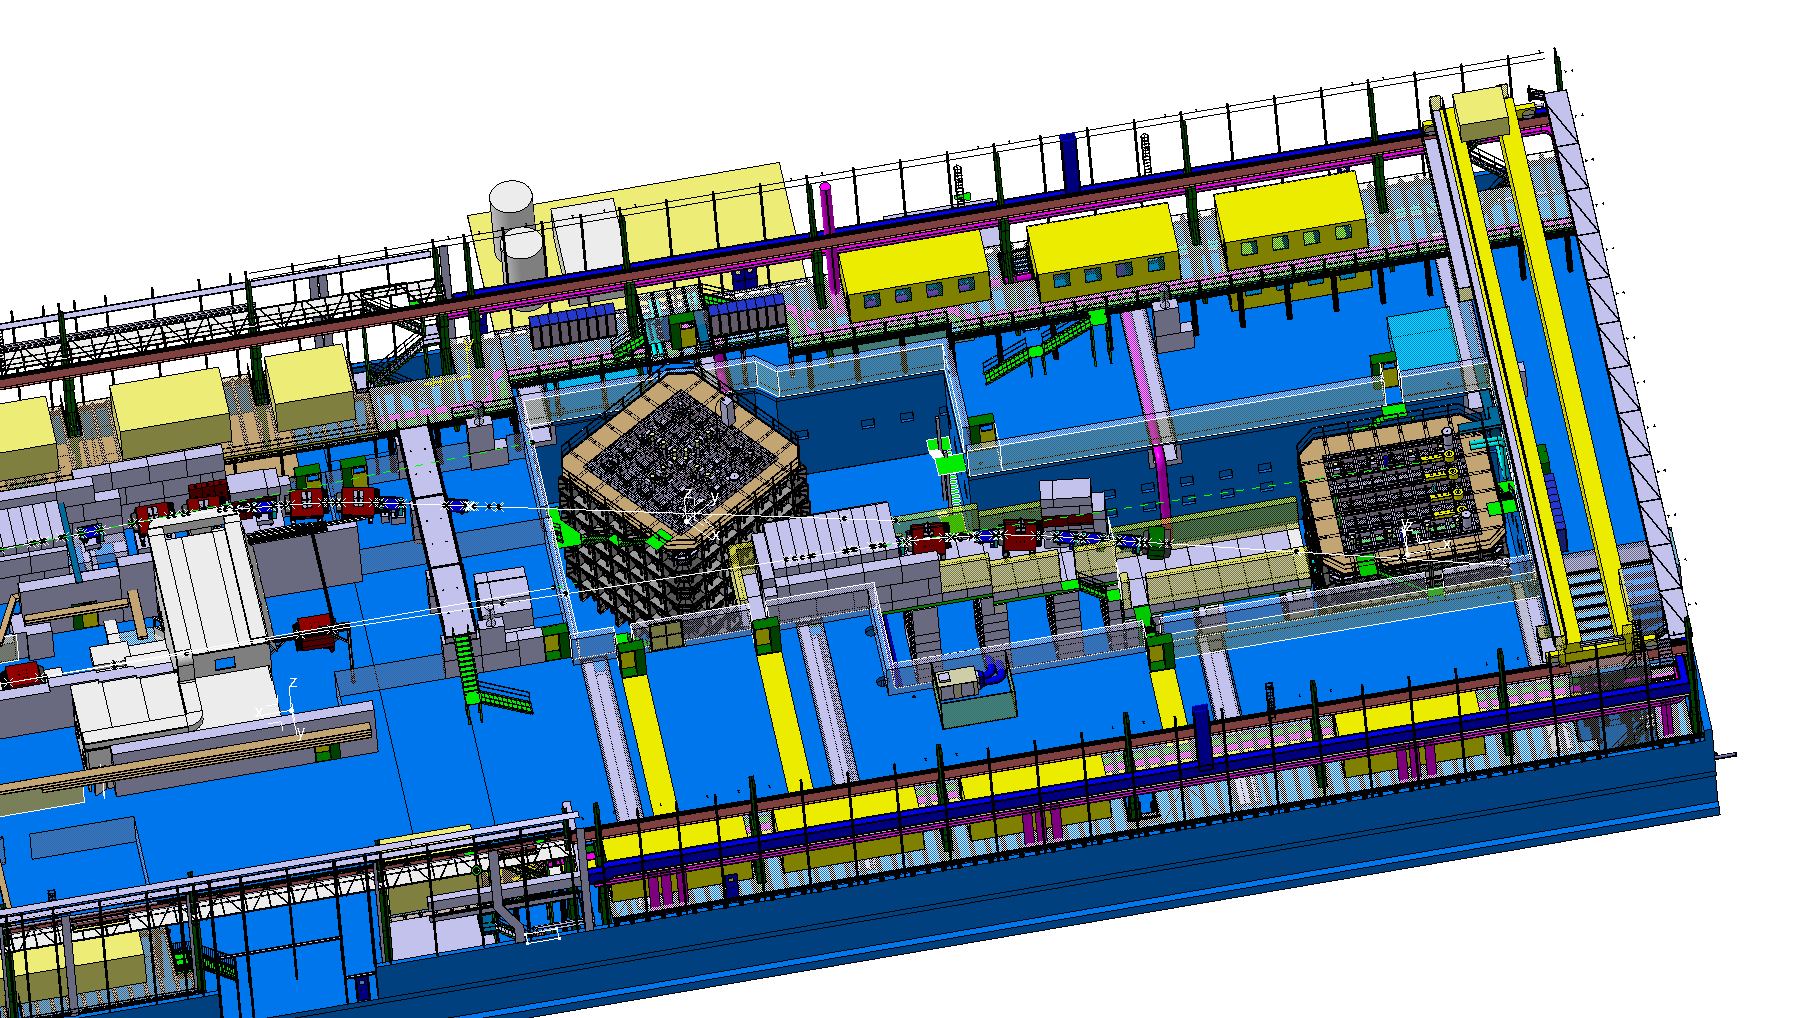
\includegraphics[width=1.0\textwidth]{np02np04.png}
\caption{\label{fig:np02np04}Diagram of the layout of the CERN north area with
  location of the protoDUNE dual phase detector (center) and the single
  phase detector (right). The direction of the particle beam is from left to right.}
\end{figure}


In the following we shall focus on the single-phase prototype which will be referred to as ``protoDUNE-SP''.
It has also received the official CERN designation as the CERN experiment NP04.
This device is essentially an ionization chamber in which Liquid Argon serves both as the target and
the sensitive medium with which to detect and measure ionization, with subsequent full 3D resonstruction of
events of interest. To this end, it is instrumented with a large number
of wire sensors immersed in Liquid Argon and grouped into planar arrays (termed Anode Plane Assemblies, or APAs).
Each face of the APA contains
two induction planes and one collection plane, in a stereo angle configuration.
The \pd-SP LArTPC will contain six APAs of the same design as in the DUNE
experiment, and of the same size which is 6$\times$2.4\,m. The maximum electron drift distance (i.e. the span between
the cathode and the APA) is 3.6\,m
and the drift field 500\,V/cm. The fiducial volume of Liquid Argon in the detector
is approximately 7.2$\times$7.2$\times$6.0\,m$^3$. The cryostat is shaped as a cube
with $\sim$11\,m side (external dimensions).
The detector features the ``cold electronics'' design
in which the amplifiers and digitizers are placed within the cryostat and operate at
cryogenic temperatures. Digital signals are fed to the Warm Interface Boards located
outside of the cryostat on its top surface and then transmitted to the Data Acquisition
System via a fiber optic line.

An important part of the DUNE design which is also included in \pd-SP is the Photon Detector capable
of providing an accurate measurement of the event timing. The components of this detector are integrated
into the APAs.

In order to implement the Cosmic Ray Trigger an external system of scintillation counters is installed
outside of the cryostat. The signals from the counters are used in the trigger logic and are also
read out and also included in the overall data stream created by the DAQ.

The \pd-SP measurement program requires characterization of the beam particles (including tracking) and adequate triggering
capabilities. The beamline used in the experiment is instrumented with fiber tracking devices, Time-of-Flight and
Cherenkov counters.
% These detectors are read out separately and their respective data is transmitted to the



%%%%%%%%%%%%%%%%%%%%%%%%

\section{Raw Data Parameters in protoDUNE-SP}
\label{sec:np04_data_rate}
\begin{table}
\begin{center}
\caption{\label{table:np04_data_rate}
  protoDUNE-SP readout parameters}
\ \\
\begin{tabularx}{0.75\textwidth}{ X  >{\setlength{\hsize}{0.8\hsize}}r}
\hline
Detector Parameter & Target \\
\hline
TPC channel count & 15,360 \\
Digitization frequency & 2\,MHz \\
Nominal electron drift time & 2.2\,ms\\
Nominal electron drift velocity & 1.6\,mm/$\mu$s\\
Readout window & 5\,ms \\
SPS spill time& 4.8\,s\\
SPS cycle& 22.5\,s\\
Nominal trigger rate & 25\,Hz \\
Single readout size (per trigger) & 230.4\,MB \\
Lossless compression factor (estimated) & 4 \\
Instantaneous data rate (in-spill) & 1440\,MB/s \\
Average data rate & 300\,MB/s \\
Total data recorded (beam + cosmic) & 3\,PB\\
Buffer to store 3 days worth of data & 300\,TB\\
\hline
\end{tabularx}
\end{center}
\end{table}

The DUNE/\pd single-phase LArTPC design has a fine spatial resolution (with wire pitch of $\sim$\,5mm)
and thus a high channel count. The 2\,MHz digitization frequency provides similarly fine
% spatial and temporal
resolution along the drift axis of the detector. The readout window is  set to 5\,ms 
based on the nominal scale of electron drift time across the active volume (2.2\,ms) to allow for detection
of ionization immediately before and after the event of interest.  These characteristics are typical of
similar modern Liquid Argon TPC detectors. The principal parameters which define the expected data rate and
volume in protoDUNE-SP are presented  in Table\,\ref{table:np04_data_rate}.


Combination of the high channel count, projected trigger rate, digitization frequency
and the relatively long readout window leads to a substantial data rate and volume. It has been decided that only
lossless compression will be applied to the data. Based on the experience of the $\mu$BooNE experiment \cite{uboone}
the lossless compression factor is conservatively estimated as $\sim$4. This also implies that before any processing can
take place the data will have to be decompressed.

The \pd-SP Data Acquisition System (DAQ) is writing data to a high performance attached storage system capable of reliably handling the data
rates as outlined in Table\,\ref{table:np04_data_rate}. From that point it is transferred to the CERN Central Storage
Facility which includes the high-performance distributed disk storage (EOS) and the tape archive (the CASTOR
system at CERN) \cite{castoreos}. The data is then transmitted to Fermilab where the bulk of offline processing
will take place.
All these transfers are managed by an automated service based on \textit{Fermi-FTS} \cite{sam,fts}.

\section{Data Quality Monitoring}
The protoDUNE-SP experiment will use an Online Monitoring system which obtains its input data directly
and in real time from the DAQ.
% Data Acquisition System.
 Its function is provide a very quick assessment of the general detector conditions
and to ascertain proper functioning of the readout chain. Online Monitoring characterized by low latency, high bandwidth
and limited CPU resources (located in the vicinity of the detector). This puts restrictions on what types of processing
can be usefully accomplished in this environment.
In order for more complex metrics to be calculated and actionable information to be provided to the experiment operators
(such as estimations of the Liquid Argon purity, signal characteristics after noise reduction, correlations of channel noise etc) 
the experiment will have a separate Data Quality Monitoring (DQM) system which complements the Online Monitoring.
This is similar to many High-Energy Physics experiments which implement ``express streams'' to perform
preliminary calculations on the data almost immediately after it leaves the DAQ. DQM is characterized by more relaxed
requiremens regarding latency of processing (which can take tens of minutes) and higher scalability, allowing
utilization of resources such the CERN Tier-0 computing facility.
%The \pd-SP DQM
It will include tasks such as
\begin{itemize}
\item Signal Processing (noise reduction, deconvolution) and basic Visualization in 2D projections
\item Liquid Argon purity monitoring using cosmic $\mu$ tracks
\item Basic monitoring of the Beam Instrumentation devices
\item Matching of beam particle tracks to signals deteected in the TPC
\end{itemize}

\noindent As an example, the workflow described in the first item in the list above can be modeled as a Directed Acyclic Graph (DAG)
is illustrated in Fig.\ref{fig:dag1}. It contains data decompression and histogramming (``ADC''), Fast Fourier Transform stage (``FFT''),
application of digital filters and deconvolution algorithms and finally the visualization stage. Each stage in the diagram may produce
numerical and graphic data (labeled ``vis product'' in the diagram) a fraction of which will be persisted in long-term storage for
later reference and debugging.

%%%%%%%%%%%%%%%%%%%%%%%%
\begin{figure}[tb]
\centering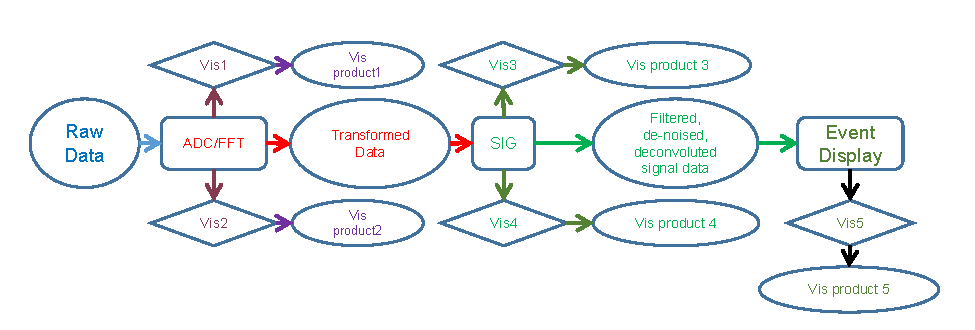
\includegraphics[width=1.0\textwidth]{dag1.pdf}
\caption{\label{fig:dag1}An example of the Data Quality Monitoring workflow}
\end{figure}
%%%%%%%%%%%%%%%%%%%%%%%%

\section{Requirements and Assumptions for the Prompt Processing System}
In order to support the Data Quality Monitoring and 
to provide automation, efficiency of operation and optimal user experience
%handle similar computational tasks which require fast turnaround during data taking,
the ``\pd Prompt Processing System'' (abbreviated as \textit{p3s}) has been developed
based on the following requirements:
%. The requirements to that system include
\begin{itemize}
\item maximal simplicity of deployment and maintenance

\item high degree of automation

\item support of computational workflows and their prioritization

\item sufficient monitoring capabilities in order to manage and track execution of workflows and ensure quick
reponse and corrective actions from the experiment operators
\end{itemize}

\noindent The prompt processing system as described here differs from a typical Workload Management System in a few important
aspects, such as
\begin{itemize}
\item the data is assumed to be accessible transparently i.e. either reside in a filesystem mounted on the p3s worker nodes,
or available via XRootD \cite{xrootd}; this means that data transport aspect in p3s is minimal

\item to ensure guaranteed execution of high-priority workflows certain jobs and workflows can be automatically
removed from the processing pool (i.e. partial loss of results is acceptable depending on the choice of policy)

\end{itemize}

\section{The Pilot Framework}
Conceptually p3s is similar to pilot-based Workload Management Systems such as Panda \cite{panda}, Dirac \cite{dirac} and others.
In this approach, a pilot job (sometimes called an \textit{agent}) is submitted to a worker node either using a local batch system,
or via the Grid, or using any other available submission mechanism. There is no dependence on the type of the local batch system
apart from the pilot submission aspect. The pilot can contain useful functionality such as validation of the environment and input data,
checking storage availability etc. Subsequently, the pilot connects to the p3s server via HTTP and requests a job to execute.

Jobs descriptions are registered in the p3s database as entries containing all necessary information -- such as the path to the executable
and the configuration file, additional environment variables that need to be set etc. These entries are created independently from pilots by
external clients such as the CLI-based client actuated by the user on a remote machine or an agent process which automatically creates
job descriptions triggered by arrival of fresh data. All interaction with the server is via HTTP in this case as well.

Upon receiving a request from a pilot job the server picks a job from the database (effectively a queue) based on priorities
and responds to the pilot with a message containing the job description. The pilot parses the message (which arrives in JSON
format) and initiates the execution. It also periodically checks the state of the job under its management, sending periodic
heartbeats to the server. Once the job completes, the pilot repeats the cycle. Its lifetime is usually set to be much larger
than typical execution time of jobs run in the system so the next job starts very quickly and avoids the latency
that may exist on the underlying batch system.

If the server does not receive heartbeats from the pilot (e.g. due to the pilot exhausting the time allotted by the batch queue)
within a period of time over a certain limit such pilot and the job under its management are declared ``timed-out'' and marked
in the database correspondingly. There is a separate process that checks pilot population in p3s and automatically
submits fresh pilots to keep it at the required level.

\section{Services, Interfaces and Component Reuse}
%Individual jobs as well as workflows (in the form of a GraphML-formatted file) are submitted by users
%by running a local client which uses HTTP to connect to the p3s server. Likewise, maintenance functions
%(e.g. puring of completed entries, collecting metrics etc) are implemented trough the HTTP interface.

The client-server architecture is used. The p3s server is implemented as a Django \cite{django} application
with standard components such as Apache Web server and PostgreSQL RDBMS as the backend storage
(a few other RDBMS can be used as well). All interactions with the server
are conducted via HTTP. The server provides monitoring capabilities by allowing the user to browse and navigate
tabulated data describing the state of the various objects in the system (e.g. pilots, jobs, data files etc).
The design of monitoring pages leverages the well known ``django-tables2'' package which results
in a very small amout of application code.

A suite of CLI clients is provided for managing pilots, jobs and
other components. In case interaction with the server requires exhange of messages these are
formatted as JSON. Workflows (DAGs) can be described in a standard format (GraphML) which is parsed
using the popular NetworkX Python module, again minimizing the application code.

%Emphasis is made on using standard, high quality packages
%(such as for parsing graph and JSON data and table rendering) so the amount of the application code is
%failry minimal.

\section{Deployment}
The \pd Prompt Processing System has been deployed at CERN, with the Web and database services running
on the CERN OpenStack virtual machines (CentOS 7). Installation of the server and client application
software is straightforward since it is Python code which can be pulled from a repository or installed from a tarball.
Python 3.5 is required.
% (mainly due to the recent version of Django on which p3s is based).
% which is different from the system version and must be installed (compiled) separately.
Since it has to be installed in the user space on the client machines  at CERN (such as running the CLI interface)
due to the site policy the Python \textit{virtual environment} appears to be the optimal solution. The CERN-supported
``acrontab'' utility which is equivalent to Unix crontab but is optimized for a large Kerberos-authenticated cluster
is used to perform periodic maintenance tasks in p3s.

At the time of writing p3s is running continuously on the \textit{lxbatch} facility at CERN. To date, tens of thousands of test jobs have run.
Scalability tests are under way utilizing realistic payload jobs developed for \pd.


\begin{thebibliography}{99}



\bibitem{cdrVol1}
R. Acciarri et al.
\emph{Long-Baseline Neutrino Facility (LBNF) and Deep Underground Neutrino Experiment (DUNE) Conceptual Design Report Volume 1: The LBNF and DUNE Projects}.\\ ~e-Print: arXiv:\textbf{1601.05471}
 %DUNE CDR Vol 1 -- The LBNF and DUNE Projects.~e-Print: arXiv:1601.05471
%\url{http://arxiv.org/abs/1601.05471}

\bibitem{cdrVol4}
R. Acciarri et al.
\emph{Long-Baseline Neutrino Facility (LBNF) and Deep Underground Neutrino Experiment (DUNE) Conceptual Design Report, Volume 4: The DUNE Detectors at LBNF}.\\~e-Print: arXiv:\textbf{1601.02984}
%\url{http://arxiv.org/abs/1601.02984}


\bibitem{uboone}
B. Jones et al.  \emph{The Status of the MicroBooNE Experiment.~J. Phys.: Conf. Series.} Vol.\textbf{408}. IOP Publishing, 2013,
doi:10.1088/1742-6596/408/1/012028

\bibitem{castoreos}
 L. Mascetti et al. \emph{Disk storage at CERN.~J. Phys.: Conf. Series.} Vol.\textbf{664}. IOP Publishing, 2015,
doi:10.1088/1742-6596/664/4/042035


\bibitem{sam}
R. A. Illingworth \emph{A data handling system for modern and future Fermilab experiments.~J. Phys.: Conf. Series.} Vol.\textbf{513}. IOP Publishing, 2014,
doi:10.1088/1742-6596/513/3/032045

\bibitem{fts}
A. Norman \emph{The Fermilab File Transfer System}.~e-Print: FNAL CD-DocDB-5412


\bibitem{xrootd}
L. Bauerdick et al. \emph{Using Xrootd to Federate Regional Storage.~J. Phys.: Conf. Series.} Vol.\textbf{396}. IOP Publishing, 2012,
doi:10.1088/1742-6596/396/4/042009

\bibitem{panda}
T. Maeno et al. \emph{Overview of ATLAS PanDA Workload Management.~J. Phys.: Conf. Series.} Vol.\textbf{331}. IOP Publishing, 2011,
doi:10.1088/1742-6596/331/7/072024



\bibitem{dirac}
A. Casajus et al.  \emph{DIRAC Pilot Framework and the DIRAC
Workload Management System.~J. Phys.: Conf. Series.} Vol.\textbf{219}. IOP Publishing, 2010,
doi:10.1088/1742-6596/219/6/062049

\bibitem{django}
N. George \emph{Mastering Django: Core. The Complete Guide to Django 1.8 LTS}~ GNW Independent Publishing, ISBN: 099461683X



\end{thebibliography}

\end{document}
